\documentclass[dvipdfmx,uplatex]{jsarticle} 
\usepackage{amsmath,amssymb}
\newcommand{\bi}{\bfseries\itshape}
\usepackage{mathrsfs}
\usepackage[multi,deluxe]{otf}
\usepackage [top=20truemm,bottom=20truemm,left=20truemm,right=20truemm]{geometry}
\usepackage[dvipdfmx]{graphicx}
\usepackage{ulem,xcolor,ascmac,pxrubrica,url}
\graphicspath{{./pic/}}

\usepackage{color}
\usepackage{xcolor}
\definecolor{lgray}{gray}{0.95}
\definecolor{lorange}{rgb}{254,216,177}
\definecolor{lgreen}{rgb}{208,233,198}
\definecolor{lpurple}{rgb}{225,176,255}
\definecolor{darkgreen}{rgb}{0.0, 0.2, 0.13}
\usepackage{threeparttable}
\usepackage[edges]{forest}
\usepackage{enumerate}
\usepackage[dvipdfmx]{hyperref}
\newcommand{\lambdabar}{\lambda \kern -0.5em\raise 0.5ex \hbox{--}}
\usepackage{lipsum} 

%\bibliographystyle{unsrt}
\bibliographystyle{mod_apsrev4-2}

\hypersetup{
    colorlinks=true,
    citecolor=red,
    linkcolor=red,
    urlcolor=blue}

\title{ChiEFTint.jl:相互作用生成コード}
\author{Sota Yoshida}

%\renewcommand{\baselinestretch}{1.2}
%\renewcommand{\headfont}{\mgfamily\propshape}

\begin{document}

\maketitle

カイラル有効場理論の相互作用を生成するJuliaコード、ChiEFTint.jlについて、概要や使い方をまとめる。

このコードは主として
\begin{itemize}
\item Entem-Machleidt型の2体力~\cite{EMrev}
\item 運動量空間でのSRG(Similarity Renormalization Group)変換
\item Fermi gas近似による有効2体化3体力~\cite{Kohno13,Kohno17err, SY_MBPT}
\item valence系の演算子を含むNN相互作用~\cite{Lukas18}
\item IMSRG計算を用いた3体力LECsのベイズ最適化
\end{itemize}
などの計算が可能で運動量空間や殻模型計算用の相互作用ファイル(KSHELL/ShellModel.jl用)を生成することができる\footnote{ココで言う「殻模型計算の相互作用ファイル」は自由空間の相互作用の意味で、基本的に、殻模型でそのまま使ってもしょうがない。模型空間用の相互作用がほしければ、MBPT(EKK)やVS-IMSRGなど別途計算が必要。}。



\section{Julia環境の準備}

Juliaのバイナリをダウンロードするか、Unix(Mac)/Linux環境ならwgetなどを使えばよい。

2021年10月16日現在の最新版はv1.6.3で、

\colorbox[gray]{0.9}{\path{$}wget \path{https://julialang-s3.julialang.org/bin/linux/x64/1.6/julia-1.6.3-linux-x86_64.tar.gz}}
を実行し展開した後、\path{julia-1.6.3/bin/julia}にエイリアスを貼るなどすれば良い。

\subsection{REPL}
上記の実行ファイルを実行すると、JuliaのREPL(対話的な実行環境)が開く。

Pythonの対話モードのように使える。

\subsection{パッケージ}
JuliaにはPythonで言うpipのようなパッケージ管理システムが用意されている。


REPL内で$]$を押すと、pkgモードになり
\colorbox[gray]{0.9}{\path{$}add packagename}で任意の公式パッケージを導入できる。

特に指定しなければ通常homeディレクトリの直下に\path{.julia}というフォルダが作成され、自身が導入したパッケージなどが入る。

スパコンの計算ノードなどで自前のJuliaを使う際、計算ノード上からみたパス\path{~/}にアクセス権限がない場合がある。
その場合は、計算ノードから見えるworkingディレクトリなどに\path{.julia}を置いておいて
\colorbox[gray]{0.9}{\path{export JULIA_DEPOT_PATH="/work/xx/yy/.julia"}}
を実行するなりジョブスクリプトに書いて置けばよい。

ちなみに\colorbox[gray]{0.9}{\path{~/.julia/environments/v1.6/Project.toml}},
\colorbox[gray]{0.9}{\path{~/.julia/environments/v1.6/Manifest.toml}}
に、インストールしたパッケージの名前とUUID,依存関係がまとめられている。

自作パッケージXXを作る際には\colorbox[gray]{0.9}{\path{Project.toml}},
\colorbox[gray]{0.9}{\path{Manifest.toml}}
を置くことで、XXを使う際には自動で開発者の環境が再現でき依存関係等を
ユーザーが気にしなくても良いようになっている。

また、任意のディレクトリに独立したJuliaのパッケージ環境を構築することもできる\footnote{Julia in Physics2021における佐藤建太氏の\href{https://youtu.be/4QBiTilaGgw?t=1609}{講演動画}がわかりやすい}。

\section{ChiEFTint.jlの概要}

\subsection{準備}

GitHubからクローンする\footnote{\today 現在はコードはpublicではなく欲しい方にのみ提供、としている}

\colorbox[gray]{0.9}{\path{$}git clone \path{https://github.com/SotaYoshida/ChiralEFTint.jl}}

次に

\colorbox[gray]{0.9}{\path{$}cd \path{ChiEFTint.jl}},
\colorbox[gray]{0.9}{\path{$}julia \path{src/package_install.jl}}

を実行し使用しているパッケージをインストールする。
\footnote{本来はパッケージ化して前述のProject/Manifest.tomlで自動で依存関係を整えるのが望ましいが簡単のためこの方法を採用している}

\colorbox[gray]{0.9}{\path{$}julia -t 12 samplerun.jl}
などと実行すると相互作用ファイルの生成ができる(はず)\footnote{Juliaではコマンドラインで-t オプションをつけるだけで使用するスレッド数を指定することが出来る}。

\subsection{インプット/ソースファイルの概要}

\path{ChiEFTint.jl/samplerun.jl}に引数無しの\path{make_chiEFTint()}という関数がある。
\path{make_chiEFTint()}の実行時には、\path{ChiEFTint.jl/parameters.jl}で指定したパラメータ($e_\mathrm{max}$や$\hbar\omega$など)が使用される。ユーザーは主に\path{ChiEFTint.jl/parameters.jl}のみを編集すれば良い。
またcoupling constants/Low-energy constants (LECs)は\path{ChiEFTint.jl/LEC.jl}にある\footnote{constを使ってglobal変数として与えている。一方で、実際の寄与を計算する各種関数の中ではLECsという辞書の値を参照して使っている。LECsを自分で最適化したりしたければ、辞書の対応するものの値を更新するように使えば良い。}。

それぞれのファイルの簡単な説明やディレクトリ構造は図~\ref{fig:dir}の通り:

\begin{figure}[h]
\begin{minipage}{0.3\linewidth}
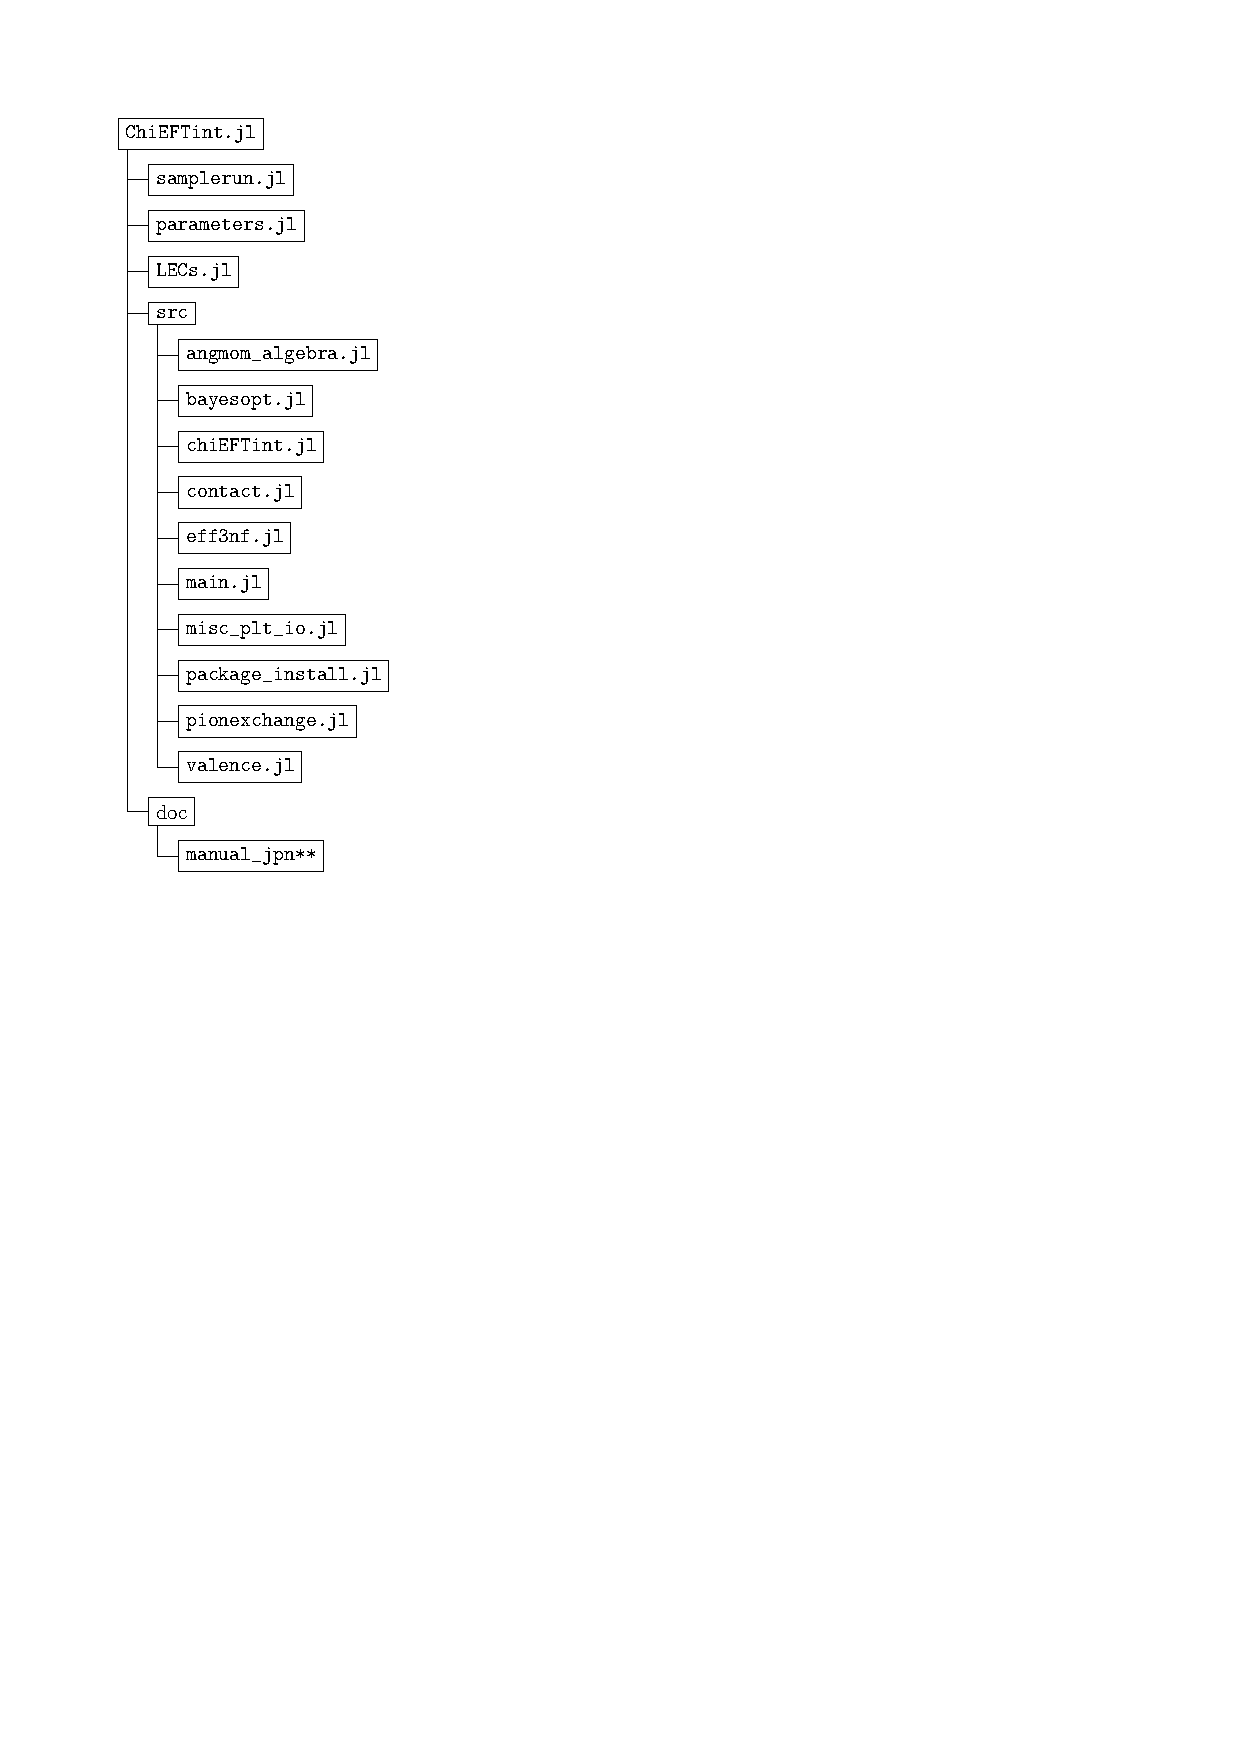
\includegraphics[width=4cm]{dirtree}
%\begin{forest}
% for tree={grow'=0,folder,draw}
% [\path{ChiEFTint.jl}
% [\path{samplerun.jl}]
% [\path{parameters.jl}]
%  [\path{LECs.jl}]
%  [\path{src}
%[\path{angmom_algebra.jl}]
%[\path{bayesopt.jl}]
%[\path{chiEFTint.jl}]
%[\path{contact.jl}]
%[\path{eff3nf.jl}]  
%[\path{main.jl}]   
%[\path{misc_plt_io.jl}]
%[\path{package_install.jl}]
%[\path{pionexchange.jl}]
%[\path{valence.jl}]]  
%  [doc
%   [\path{manual_jpn**}]
%  ]
% ]
%\end{forest}
\end{minipage}
\begin{minipage}{0.6\linewidth}
\begin{tabular}[t]{ll}
\path{angmom_algebra.jl} & 角運動量関連やHOB(Talmi変換)の計算\\
\path{bayesopt.jl}& IMSRG+ベイズ最適化のための部分 \\
\path{chiEFTint.jl}& モジュールファイル(使用パッケージの指定,関数のexport)\\
\path{contact.jl}& contact項の寄与の計算 \\
\path{eff3nf.jl}  & 有効2体化3体力の計算\\
\path{main.jl}& main部分\\
\path{misc_plt_io.jl}& お絵かきやI/O関係 \\
\path{package_install.jl}& 使用パッケージのインストール用\\
\path{pionexchange.jl}& pion交換項の寄与の計算\\
\path{valence.jl} & バレンス系演算子の寄与の計算
\end{tabular}
\end{minipage}
\caption{階層構造とsrcファイルの説明\label{fig:dir}}
\end{figure}


\newpage

\bigskip 





\section{ユーザーが指定すべきパラメータ}

\path{parameters.jl}の中にあるパラメータのうち、通常の用途で変更すべきものは以下の通り
\begin{table}[h]
\begin{threeparttable}[h]
\begin{tabular*}{16cm}{lllll}
変数名 & 値の例  & 説明 \\ 
\hline \\
\path{n_mesh} &  40  & 運動量メッシュ点の数 \tnote{a}  \\
\path{emax}  & 8 & harmonic oscillatorのmajor shellの数  \\
\path{chi_order} & 3 & カイラル摂動論の次数(正確には非ゼロの寄与をする次数, N3LO=3) \\
\path{calc_NN} & true/false & Entem-Machleidt型2体力の計算\\
\path{calc_3N} & true/false &有効2体化3体力の計算\\
\path{kF} &1.35 &有効2体化3体力の計算に使うFermi momentum\\
\path{hw} & 20.0 & harmonic oscillatorのパラメータ $\hbar\omega$ \\
\path{Anum} & 4 & 質量数 ($\hbar\omega$を公式で決めずに手で入れるなら使用しない) \\
\path{srg} & true/false & 運動量空間でのSRG変換を行うかどうか \tnote{b} \\
\path{srg_lambda} & 2.0 & SRG変換のパラメータ $[fm]^{-1}$ \tnote{c} \\
\path{tbme_fmt} & \path{"snt"/"myg"} & 相互作用フォーマット\tnote{d}\\
\path{target_nlj} & [ ] & 興味のある軌道($[[n,l,j]]$)のリスト\tnote{e} \\
\path{v_chi_order} & 0 & (NLO=1)バレンス系の演算子の項を計算 \tnote{f} \\
 \hline
\end{tabular*}
\begin{tablenotes}
\item[a] TBME生成には40もあれば精度は十分だが、運動量空間で見栄えの良い図が書きたければ100-200にすると良い。ただし、その分SRG変換などは遅くなる。
\item[b] 今の実装ではinduceされる多体力は考慮していない(いわゆるNN-onlyに相当)
\item[c] IMSRGなどの文献では良く$s=1/\lambda^{4}$が用いられる
\item[d] snt形式(KSHELL/ShellModel.jlのインプット)か、myg(\href{https://orcid.org/0000-0002-6529-4164}{Takayuki Miyagi})形式
\item[e] 該当するものだけをトリミングしてくれるはずだが...限られた例でしか確認していないので注意が必要
\item[f] 未チェックなので、使用は非推奨, N3LO=3は未実装
\end{tablenotes}
\end{threeparttable}
\end{table}



\section{LECs}

\path{ChiEFTint.jl/LECs.jl}にはLow-energy constantsがまとめられている。

2体力についてはEntem Machleidtのレビュー~\cite{EMrev}にある値を使用しているが、
NNLO3体力で初めて現れる$c_D,c_E$については適当な値を取っている。

とくに2体力は基本固定して使うことを想定しているが、前述のようにLECsを自分で最適化したりしたければ、\path{ChiEFTint.jl/src/main.jl}を書き換えれば良い\footnote{induceされる多体力を無視しているので、むしろ$\mathrm{NNLO}_\mathrm{sat}$のような哲学でLECsを決めるのもよいかもしれない}。
より具体的には、\path{ChiEFTint.jl/src/main.jl}内の\path{make_chiEFTint}関数の後半部分に、IMSRG計算を用いたベイズ最適化のコードが書いてあるので、それに倣って別の方法で最適化する関数を挿し込めば良い。

\bibliography{manual_jpn}

\end{document}